%
%  This is an example LaTeX file. The percent sign is used to mark the
% start of a comment.
%
%  - Michael Weeks, January, 2003
%
\documentclass[conference]{IEEEconf}
\usepackage[dvips]{graphics}
\usepackage{tikz}
\usepackage{dtklogos}
\usepackage[utf8]{inputenc}
\usetikzlibrary{mindmap}
\usepackage[hidelinks,pdfencoding=auto]{hyperref}
% Information boxes
\newcommand*{\info}[4][16.3]{%
  \node [ annotation, #3, scale=0.65, text width = #1em,
          inner sep = 2mm ] at (#2) {%
  \list{$\bullet$}{\topsep=0pt\itemsep=0pt\parsep=0pt
    \parskip=0pt\labelwidth=8pt\leftmargin=8pt
    \itemindent=0pt\labelsep=2pt}%
    #4
  \endlist
  };
}

\begin{document}
  \title{My Example LaTeX Conference Paper}
  \author{Michael Weeks \\
  \begin{affiliation}
   Computer Science Department\\
   Georgia State University\\
   Atlanta, Georgia, USA 30303\\
\end{affiliation} \\
\email{mweeks@nospam.org}
}
  \maketitle


\begin{abstract}
This is the abstract. You can use this file to start your own LaTeX file,
and just delete the stuff you do not need. \LaTeX  is a lot like working
with HTML: you can specify where text effects begin, and where they end.
\end{abstract}

\section{Introduction}\label{sec:intro}
Here is the introduction.
Since there is no blank line between these first 3 sentences, they are 
treated as one paragraph. 
Here is a vertical space (of 0.3 inches):
\vspace{.3in}

And here is a \hspace{.3in}horizontal space (of 0.3 inches).

A blank line means that the last paragraph is over, and it is time to start
a new one.

You can have text in {\it italics} font, or in {\bf bold} font,
\underline{underlined}, and even $\overline{overlined}$.
What if you want overlined text, without italics? This can
be done by using \verb"mathrm" in the 
$\overline{\mathrm{overlined}}$ specification.




\begin{table}[!hbt]
\begin{center}
  \caption{Table captions go above tables.}
  \vspace{0.2in}
  \begin{tabular}{|r|c|c|c|}
     \hline
 & runs & hits & errors  \\
     \hline
Cardinals  & 2 & 2 & 1  \\
Panthers & 4 & 8 & 0  \\
Tigers  & 2 & 3 & 2  \\
Braves  & 3 & 10 & 3  \\
     \hline
  \end{tabular}
  \label{tab:example_tab}
\end{center}
\end{table}

What if you want to include a figure? 
Here is an example, figure~\ref{fig:phasor1}, that is saved in 
encapsulated postscript format.




Skip a lot of space  \bigskip  vertically.
\begin{figure}[h]
\centering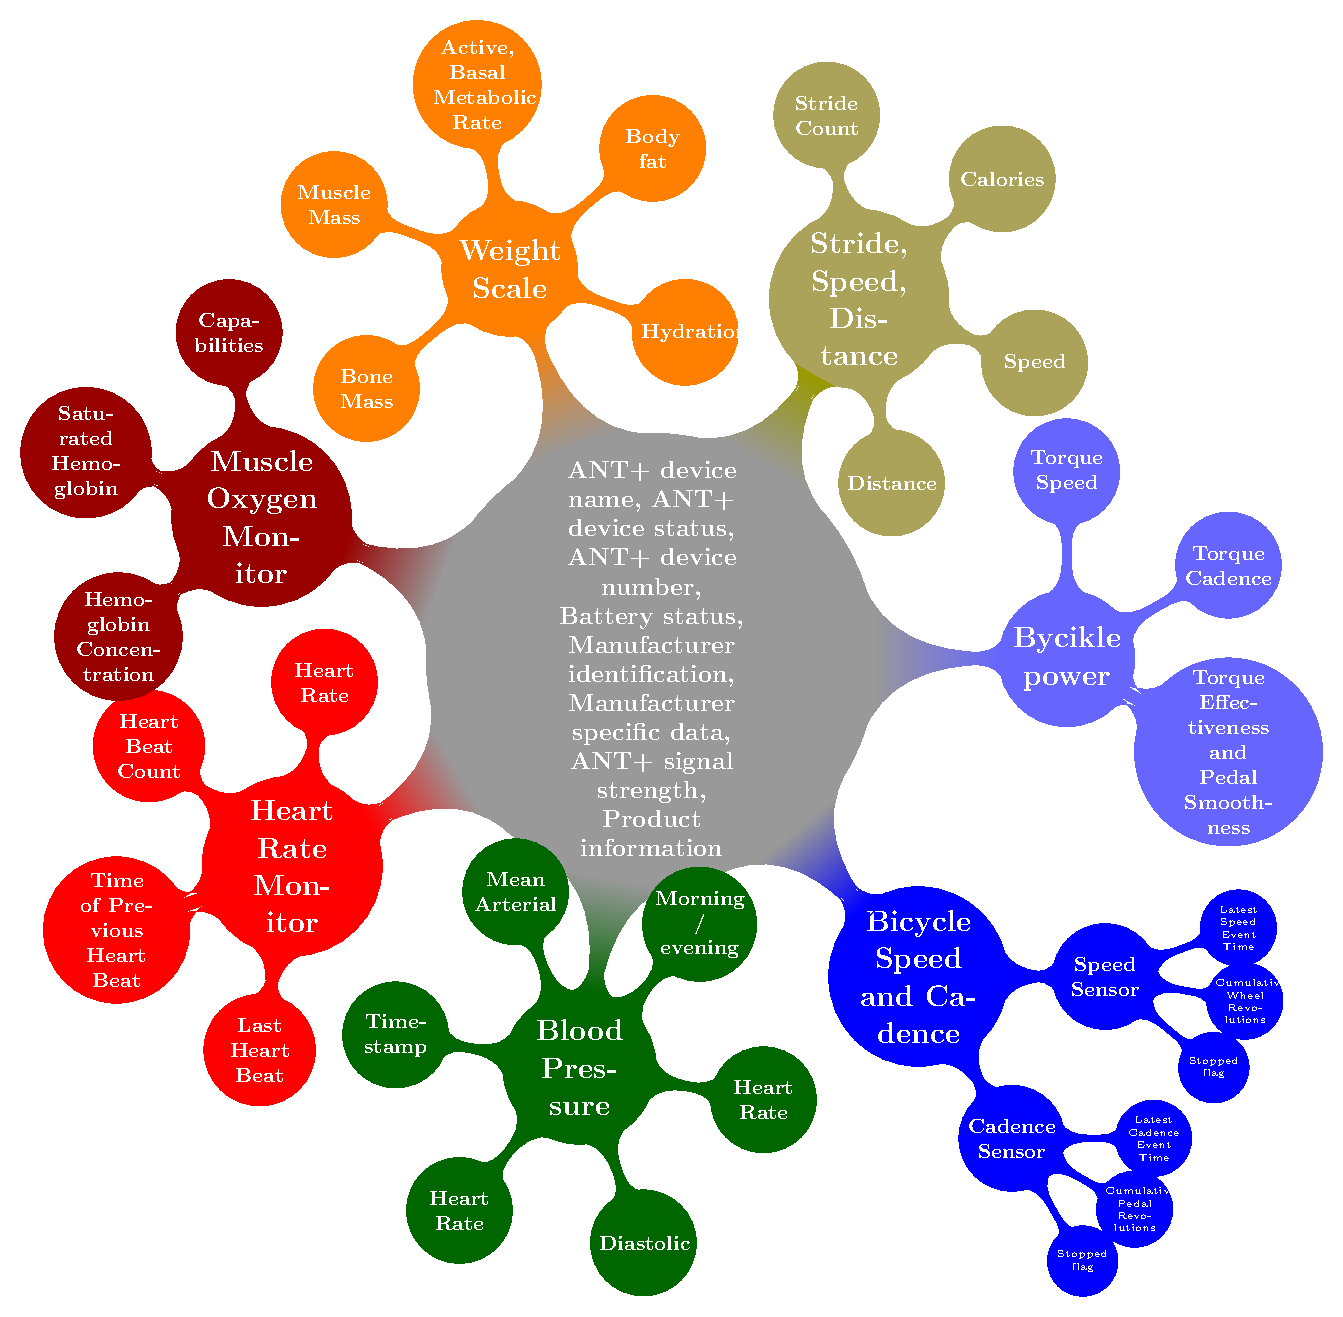
\includegraphics[width=8.50cm, height=8cm]{AntPlusProfiles}
\caption{\label{FRA}Schematic Description of the Framework.}

\end{figure}
\section{Here is some Computer Code}\label{sec:code}

I like using the \verb"verbatim" specification for computer code. 
For example, here is something that appears in several
languages:

\begin{verbatim}
    for (int i=0; i< MAXVALUE-1; i++)
    {
        if (array[i] < array[i+1]) 
        {
            temp = array[i];
            array[i] = array[i+1];
            array[i+1] = temp;
        }
    }
\end{verbatim}

See how it makes the code stand out? I think it makes it
much easier to read, too.

\section{Here is some Math}\label{sec:math}
This is different from the previous section, section~\ref{sec:intro}.
This section gives some examples of Math.



If you use a character, but LaTeX complains about it, try putting a 
back-slash before it. For example, 
f = x\^{}y  uses the carat character. 
If you want to end a line, use 2 back-slashes.
If you want the backslash character $\backslash$ in your document,
this can be done, too.

Here's an equation:

\[ M^\bot = \{ f \in V' : f(m) = 0 \mbox{ for all } m \in M \}.\]

Here's d2u/dx2 : (use the dollar sign before and after math stuff)

$ \frac{d^2 u}{dx^2} $

Here's another equation:

\[ \lim_{x \to 0} \frac{3x^2 +7x^3}{x^2 +5x^4} = 3.\]

Here's a summation:
\[ \sum_{k=1}^n k^2 = \frac{1}{2} n (n+1).\] 

and an integral:
\[ \int_a^b f(x)\,dx.\]

Here are some Greek letters:
$ \Delta \Psi \Phi $
and some lower case ones:
$ \delta \psi \phi \omega \pi \sigma \mu $.

For more info, see


http://www.maths.tcd.ie/\~{}dwilkins/LaTeXPrimer/

\section{Filler}

It is always a good idea to have text between a section header and
a subheading.

\subsection{Sentences About Nothing}

This sentence does not really say anything important, but it does take up space.
This sentence does not really say anything important, but it does take up space.
This sentence does not really say anything important, but it does take up space.
This sentence does not really say anything important, but it does take up space.
This sentence does not really say anything important, but it does take up space.

\newpage

{\bf I added a ``newpage'' command above to make the columns somewhat even.}
This sentence does not really say anything important, but it does take up space.
This sentence does not really say anything important, but it does take up space.
This sentence does not really say anything important, but it does take up space.
This sentence does not really say anything important, but it does take up space.
This sentence does not really say anything important, but it does take up space.
This sentence does not really say anything important, but it does take up space.
This sentence does not really say anything important, but it does take up space.
This sentence does not really say anything important, but it does take up space.


\subsection{More About Nothing}

This sentence does not really say anything important, but it does take up space.
This sentence does not really say anything important, but it does take up space.
This sentence does not really say anything important, but it does take up space.
This sentence does not really say anything important, but it does take up space.
This sentence does not really say anything important, but it does take up space.
This sentence does not really say anything important, but it does take up space.
This sentence does not really say anything important, but it does take up space.
This sentence does not really say anything important, but it does take up space.
This sentence does not really say anything important, but it does take up space.
This sentence does not really say anything important, but it does take up space.

This sentence does not really say anything important, but it does take up space.
This sentence does not really say anything important, but it does take up space.




% Now here is the reference section.

\begin{thebibliography}{99}

  % Book
  \bibitem{Weste93} Neil H. E. Weste and Kamran Eshraghian, {\it Principles
  of CMOS VLSI Design}, 2nd ed. Reading, MA: Addison-Wesley, 1993.

  %Example of a Conference Paper
  \bibitem{LiY88} R. A. Lincoln and K. Yao, ``Efficient Systolic Kalman
  Filtering Design by Dependence Graph Mapping,'' in {\it VLSI Signal
  Processing, III}, IEEE Press, R. W. Brodersen and H. S. Moscovitz Eds.,
  1988, pp.~396--410.

  % Example of a Journal Paper
  \bibitem{BiS92} C. H. Bischof and G. M. Shroff, ``On Updating Signal
  Subspaces,'' {\it IEEE Trans. on Signal Processing}, vol.~40, no.~1,
  pp.~96--105, Jan. 1992.

\end{thebibliography}
\end{document}